\documentclass[11pt, a4paper]{article}

\usepackage[margin=0.75in]{geometry}
\usepackage{graphicx}
\usepackage{enumerate}% http://ctan.org/pkg/enumerate


\begin{document}

\title{Task 1: Scheduling\\Design Document}
\author{}
\date{}
\maketitle


\begin{center}
Group:\\
Robert Barr, rjb19@ic.ac.uk\\
Sebastian Males, sm919@ic.ac.uk\\
Euan Scott-Watson, es1519@ic.ac.uk\\
Alex Usher, awu19@ic.ac.uk
\end{center}

\section{Priority Scheduling}
	\subsection{Data Structures}
		A1: (2 marks)\\
		Copy here the declaration of each new or changed 'struct' or 'struct' member, global or static
		variable, 'typedef' or enumeration. Identify the purpose in roughly 25 words.
		
		\begin{center}\textbf{thread.h}\end{center}
		Added to 'struct' thread:
		
		\begin{verbatim}
      int effective_priority_cache; /* Cache for calculating the effective priority.*/
        
      /* Struct members relating to donations */
      struct list donors_list;          /* Sorted list of donating threads */
      struct lock *donating_for;        /* The lock we are donating for.      
                                           Can be NULL */
      struct list_elem donation_elem;   /* list elem for donors list */
        
		\end{verbatim}
		\verb+donors_list+ holds a list of threads donating
		to the owner, tied together by \verb+donation_elem+. The member \verb+donating_for+
		represents the lock this thread failed to acquire and as a consequence, it is donating for. It can 
		be \verb+NULL+ if there is no lock being waited
		on.\\
		We use \verb+effective_priority_cache+ to compute
		the effective priority more efficiently, not having to go down the priority chain every time we want
		to fetch it.

		\begin{center}\textbf{thread.c}\end{center}
		\begin{verbatim}
		
	      /* a list to contain a queue for each priority level */
      static struct list scheduling_queues[NUMBER_QUEUES];
        
		\end{verbatim}		
        An array of queues for each priority a thread can have. Completely replaces the ready list so this was deleted. The macro \verb+NUMBER_QUEUES+ is defined
        as \verb!PRI_MAX + 1!.

    \vskip 1in

		\begin{center}\textbf{synch.c}\end{center}
		\begin{verbatim}
      /* One semaphore in a list. */
      struct semaphore_elem {
        struct thread *thread;      /* The thread that created the elem */
        struct semaphore semaphore; /* This semaphore. */
        struct list_elem elem;      /* List element. */
      };

		\end{verbatim}
		Here we have added the 'struct' member \verb+thread+ so we know the priority to sort by in the queue
		of a condition - it represents the thread that
		created this \verb+semaphore_elem+.\bigskip\\
		A2: (4 marks)\\
		Draw a diagram that illustrates a nested donation in your structure and briefly explain how 
		this works.
		
		\begin{center}
			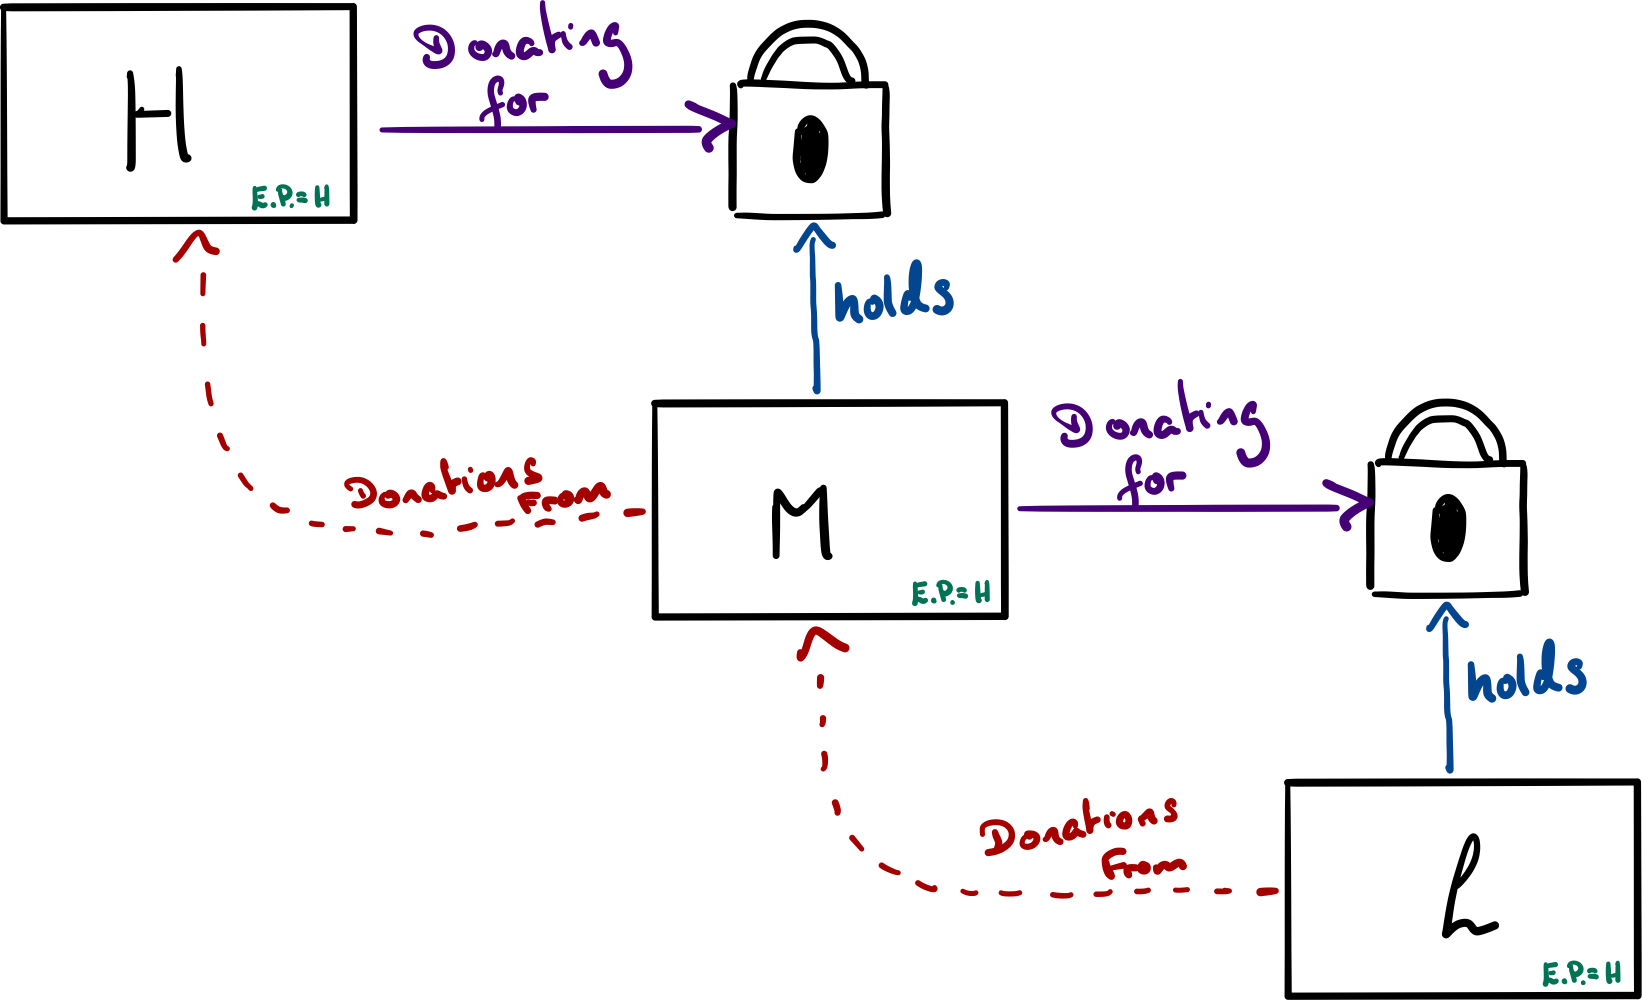
\includegraphics[width=0.7\textwidth]{Diagram.jpeg}
		\end{center}
		When H tries to acquire a lock held by M, it will add itself to the \verb+donors_list+ in M, maintaining the sorted (by effective priority) nature of the list. This will increase M's effective priority to 
    H. The same process is repeated when M tries to acquire L, and the effective priority from H cascades into L via recursion. If for instance,
		now a thread would start donating to H (priority: VH - very high), that would recursively reach M and L too. When any lock is released, the process is reverted and if that's the case, the donations are
		transfered to the next thread to acquire the lock.

	\subsection{Algorithms}
		A3: (3 marks)\\
		How do you ensure that the highest priority waiting thread wakes up first for a (i) lock, 
		(ii) semaphore, or (iii) condition variable?
		\begin{enumerate}[(i)]
		  \item To wake up the correct thread blocked at
		  a particular lock, we use the waiters list of 
		  the corresponding semaphore, which as detailed
		  below is sorted by effective priority.
		  When the lock is released, if the
		  waiters list for its semaphore isn't
		  empty, we transfer all donations to the next 
      holder (the maximum effective priority thread
      in the waiters list), before the next holder is
      set in \verb+sema_up()+.\\
		  When a thread is donating to another, the
		  effective priority could get changed, so any waiting
		  list that the thread is in now needs reordering
		  - this applies to both semaphores and conditions
		  too. We do this recursively up the donation chain
        with the function \verb+priority_reorder()+, by removing it
        from the donors list and reinserting it in order
        of its effective priority.

         \item For a semaphore, we insert the threads
         in the waiters list using
         \verb+list_push_back()+, but in order
         to unblock the right threads we then need to do a \verb+list_sort()+
         by effective priority in \verb+sema_up()+ before we choose the next thread. This would mean that 
         calling \verb+list_pop_front()+ would always get the
         highest priority thread.

        \item The condition waiters list is sorted in
          \verb+cond_signal()+ using
        a \verb+list_less_func+ called\\ 
        \verb+condition_priority_compare()+, which uses
        the effective priority of the thread in the\\
        \verb+semaphore_elem+ to sort the condition waiters
        list. This means that calling \verb+list_pop_front()+
        on signalling a condition always gets the highest
        effective priority thread.
        \end{enumerate}
		A4: (3 marks)\\
		Describe the sequence of events when a call to \verb+lock_acquire()+ causes a priority 
		donation. How is nested donation handled?\bigskip\\
		When a thread tries to acquire a lock, we have to check if the lock's semaphore has value 0. If it does, this means that another thread has acquired the lock,
    so we need to donate to the holder. To do this, we first have to set the thread's \verb+donating_for+ member to the lock. The thread
    will then insert itself into the \verb+donors_list+ of the lock holder, using the thread's \verb+donation_elem+ and the \verb+list_less_func+ \verb+donation_priority_compare()+.\\
    To handle a nested donation, we then call the function \verb+priority_reorder()+, which will recursively move down the donation chain calculating the 
    \verb+effective_priority_cache+ for each thread
    it passes through and reordering all the 
    \verb+donors_list+s, ensuring that they remain
    in descending order of effective priority.\bigskip\\
		A5: (3 marks)\\
		Describe the sequence of events when \verb+lock_release()+ is called on a lock that a 
		higher-priority thread is waiting for.\bigskip\\
    When a thread releases a lock, we have to check whether there is anything currently waiting for access to it, in the corresponding semaphore's waiters list. If 
    something is waiting for the lock - in this case the 
    higher-priority thread - then we know there is at least
    one donation to it. Before we call \verb+sema_up()+, 
    we therefore have to transfer all other donations 
    on the lock to the \verb+donors_list+ of the next
    thread to run, which would be the highest effective 
    priority thread in the semaphore waiters list (here we
    assume this is the higher-priority thread). We set 
    this thread's \verb+donating_for+ member to 
    \verb+NULL+ since it is being unblocked, and call
    \verb+invalidate_effective_priority_cache()+ on both
    the previous and next holder.
  
	\subsection{Synchronisation}
		A6: (2 marks)\\
		How do you avoid a race condition in \verb+thread_set_priority()+ when a thread needs to 
		recompute its effective priority, but the donated priorities potentially change during the 
		computation? Can you use a lock to avoid the race?\bigskip\\
		We do not need to worry about race conditions
		in \verb+thread_set_priority()+, because
		we don't recompute the effective priority
    on the spot. Since our \verb+thread_get_priority()+
		function always calculates the maximum between
		the base priority and the largest donated priority
		(\verb+effective_priority_cache+) no additional
		side-effecting steps are required. We therefore do not need
    to use a lock or any synchronisation primitive in 
    \verb+thread_set_priority()+ since there are no race conditions.

	\subsection{Rationale}
		A7: (3 marks)\\
		Why did you choose this design? In what ways is it superior to another design you 
		considered?\bigskip\\
		Our main aim throughout designing the priority
		scheduler was simplicity with little overhead
		when it comes to time complexity. Keeping the
		\verb+donors_list+ sorted assures that calls to
		\\\verb+thread_get_priority()+ are $O(1)$. This is
		important because we call this every time a 
		comparison occurs in any sorting by priority
		of the threads. Furthermore, any future
		additions to the code can utilise this function
		securely, without encountering hidden complexities.
		We could have avoided sorting in \verb+sema_up()+
		and \verb+cond_signal()+ by storing the semaphore
		and the condition the thread is blocked at and
		reinsert changed priorities in
    \verb+priority_reorder()+, but that would increase
		the complexity of the code by coupling the
		thread `struct` further without making a 
		very significant difference in time complexity (the sorted
    insert is $O(n)$ and an overall sort is $O(n \cdot log(n))$.

\section{Advanced Scheduler}
	\subsection{Data Structures}
		B1: (2 marks)\\
		Copy here the declaration of each new or changed 'struct' or 'struct' member, global or 
		static variable, 'typedef' or enumeration. Identify the purpose of each in roughly 25 
		words.
    \begin{center}
      \textbf{thread.h}
    \end{center}
		Added to 'struct' thread:
		\begin{verbatim}
      int nice;                           /* Stores the niceness of thread */
      fixed_point recent_cpu;             /* Stores the recent cpu usage of thread */     
		\end{verbatim}
		The \verb+nice+ and \verb+recent_cpu+ values are thread specific and so were stored in the thread's struct. \verb+nice+ can only be between -20 and 20 and so was stored as an integer.
    \verb+recent_cpu+ is a fixed point number and so was stored as an \verb+int32_t+ to accomodate the p.q format.
		\begin{verbatim}
		      /* Moving average of the no. threads waiting to run */
		      fixed_point load_avg;
		\end{verbatim}
		We have added a global variable: \verb+int32_t load_avg+. This is global as the load average is the same for all threads. Once again this is a fixed point number and so we used \verb+int32_t+ once again
		
		\begin{center}
      \textbf{fixedpoint.h}
    \end{center}
		\begin{verbatim}
		      typedef int32_t fixed_point;
		\end{verbatim}
		We added a typedef named \verb|fixed_point| so that it would be easier to differentiate between integers and p.q format integers in the code.
		
    \begin{center}
      \textbf{timer.c}
    \end{center}
		\begin{verbatim}
      #define PRIORITY_UPDATE 4
    \end{verbatim}
		Every 4 ticks the priority levels of all threads must be updated. We therefore created a macro for this to remove magic numbers when checking the thread count.

	\subsection{Algorithms}
		B2: (3 marks)\\
		Suppose threads A, B, and C have nice values 0, 1 and 2, and each has a \verb+recent_cpu+ value 
		of 0. Fill in the table below showing the scheduling decision, the priority and the 
		\verb+recent_cpu+ values for each thread after each given number of timer ticks:
		\begin{center}
			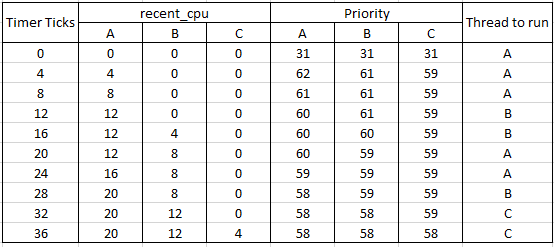
\includegraphics[width=0.7\textwidth]{table_diagram.png}
		\end{center}
		B3: (2 Marks)\\
		Did any ambiguities in the scheduler specification make values in the table uncertain? If so, 
		what rule did you use to resolve them?\bigskip\\
		The specification did not say what to do when the currently running thread has the same priority as another thread after recalculation. We decided to continue the currently running thread until the priority decreased below the next highest. This meant there was less overhead in changing the stack, program counter and registers resulting in a slightly faster execution.
	\subsection{Rationale}
		B4: (3 marks)\\
		Briefly critique your design, pointing out advantages and disadvantages in your design 
		choices.\bigskip\\
		A disadvantage of our design is that we constantly have 64 queues even if some of them are empty. Although they are doubly-linked lists and so only the head and the tail are stored, this still adds to the space complexity. \\
		We started with one schedule function to reshuffle all the threads after priority updates, however, we found that this just over-complicated things and added to the time complexity. Therefore, we 
    decided to insert the thread into the necessary queue as they were updated rather than doing it in one batch afterwards. This also ensures that threads were not scheduled multiple times as we originally 
    iterated through each queue for the re-positioning. This lead to a smaller time complexity reducing from $O(n)$ when we re-looped through the queues to $O(1)$ as we inserted each thread after updating
    its priority.
\end{document}
